\begin{pa} \label{PA:3.1}
Consider the function $h$ given by the graph in Figure~\ref{F:3.1.PA1}.  Use the graph to answer each of the following questions.
\begin{figure}[h]
\begin{center}
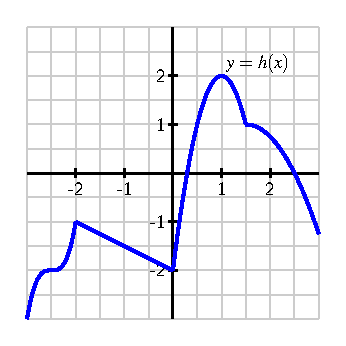
\includegraphics{figures/3_1_PA1.eps}
\caption{The graph of a function $h$ on the interval $[-3,3]$.} \label{F:3.1.PA1}
\end{center}
\end{figure}
\ba
	\item Identify all of the values of $c$ for which $h(c)$ is a local maximum of $h$.
	\item Identify all of the values of $c$ for which $h(c)$ is a local minimum of $h$.
	\item Does $h$ have a global maximum?  If so, what is the value of this global maximum?
	\item Does $h$ have a global minimum?  If so, what is its value?
	\item Identify all values of $c$ for which $h'(c) = 0$.
	\item Identify all values of $c$ for which $h'(c)$ does not exist.
	\item True or false: every relative maximum and minimum of $h$ occurs at a point where $h'(c)$ is either zero or does not exist.
	\item True or false: at every point where $h'(c)$ is zero or does not exist, $h$ has a relative maximum or minimum.
\ea
\end{pa} \afterpa